\documentclass[journal,12pt,onecolumn,draftcls]{IEEEtran}
\usepackage{amsmath,amssymb,amsfonts}
\usepackage{algorithmic}
\usepackage{graphicx}
\usepackage{xcolor}
\newcommand{\editornote}[1]{\par\textit{\textcolor{blue}{\textbf{Editor's Note:} #1}}\par}
\usepackage{float}
\usepackage{setspace}
\usepackage{hyperref}
\usepackage{makecell}

\hypersetup{
      colorlinks=true,
      linkcolor=blue,
      citecolor=black,      
      urlcolor=blue
}

\doublespacing

\begin{document}
\title{One-Class Autoencoder for Anomaly Detection of Malaria Infected Cells}
\author{\IEEEauthorblockN{Author Name}}
\maketitle
\begin{abstract}
  Malaria remains a major public health challenge, especially in developing regions where diagnostic resources are limited. Traditional detection methods often suffer from low sensitivity and require expert interpretation. In this study, we propose a one-class autoencoder trained exclusively on normal red blood cell images to learn their latent structure and identify anomalous deviations associated with malaria infection. Using structural similarity (SSIM) as the primary evaluation metric, our method demonstrates strong classification performance on two microscopy datasets. These results highlight the potential of unsupervised learning in enhancing automated malaria diagnosis, particularly in resource-constrained settings.
\end{abstract}

\begin{IEEEkeywords}
anomaly detection, malaria detection, deep learning, one class autoencoders
\end{IEEEkeywords}

\section{Problem Statement}
Malaria is a life-threatening disease caused by parasites transmitted to people through the bites of infected mosquitoes. The \textit{World Malaria Report 2022} highlights that there were an estimated 247 million malaria cases in 2021 in 84 endemic countries \cite{who2022}, with most of the increase coming from countries in the African Region of the World Health Organization (WHO). Malaria case incidence declined from 82 in 2000 to 57 in 2019, before increasing to 59 in 2020, with no change in case incidence between 2020 and 2021. The increase in 2020 was associated with disruptions to services during the COVID-19 pandemic, which led to an estimated additional 13.4 million cases between 2019 and 2021. Twenty-nine countries accounted for 96\% of global malaria cases, with Nigeria, the Democratic Republic of the Congo, Uganda, and Mozambique accounting for nearly half. The African Region, with an estimated 234 million cases in 2021, accounted for about 95\% of global cases \cite{who2022}.

Malaria continues to pose a significant public health challenge, particularly in developing countries, where access to diagnostic tools and treatment is often limited. Current diagnostic methods for malaria detection, such as microscopy and rapid diagnostic tests \cite{wilson2012}, have several limitations, including variability in diagnostic sensitivity and specificity, high costs, and dependence on skilled personnel. As such, the development of more accurate and efficient methods for malaria detection—particularly in resource-limited settings—is critical.

To address these challenges, we turn to anomaly detection, also known as outlier detection—a technique used to identify rare or unexpected observations or patterns in a dataset \cite{chandola2009}, \cite{ruff2021}, \cite{edgeworth1887}. Anomaly detection offers a promising avenue for improving malaria diagnostics. It is widely applied in fields such as finance, cybersecurity, and medical diagnosis, where identifying irregularities is critical for detecting fraud, uncovering network intrusions, or diagnosing diseases. This concept has proven useful in identifying the presence of the malaria parasite in cell images.

In this research endeavor, we propose a one-class methodology for the classification of red blood cells depicted in microscopic images. This approach leverages normal cell images to address a common challenge in medical imaging: the insufficient number of abnormal or infected instances.

One-class anomaly detection is a machine learning technique that is particularly useful for identifying anomalous instances within a single class of data. By training a model on a large and diverse dataset of normal instances, the proposed method can extract deep features that distinguish normal from anomalous cases. These features can be learned using deep learning models such as autoencoders and convolutional neural networks (CNNs), which capture hierarchical representations of image data, including both global and local patterns \cite{torres2021}.

Deep learning, which falls under the umbrella of machine learning, involves creating computer models capable of learning patterns and making predictions. What sets deep learning apart is its ability to automatically recognize important features in data without requiring experts to manually identify the most relevant information. These capabilities make deep learning especially valuable in fields like medical imaging. In areas where it is difficult to determine which parts of an image are diagnostically important—such as disease classification and tumor detection—deep learning models excel at interpreting complex data, making them powerful tools in healthcare and beyond \cite{torres2021}.

In summary, the major solutions that this proposal seeks to solve are:
\begin{itemize}
  \item \textbf{Addressing Data Scarcity:} This approach tackles the persistent challenge of limited abnormal samples in medical imaging by leveraging normal cell images to train a robust detection model.
  \item \textbf{Reducing False Positives:} The method leads to fewer false alarms—an essential benefit in domains such as medical diagnostics and fraud detection, where false positives can have serious consequences.
\end{itemize}

Through this research, we demonstrate that our one-class autoencoder achieves above-average accuracy in detecting infected cells in microscopic images. This result highlights the model’s potential as a reliable tool for improving malaria diagnosis and strengthening healthcare delivery, especially in resource-limited settings.

\section{Literature Review}
Bobde et al. \cite{bobde2022} proposed an autoencoder model for malaria cell classification. They trained the model on image data and froze the encoder to extract features. The encoder was then integrated with fully connected convolutional neural network (CNN) layers and used a softmax activation function for binary classification. After fine-tuning, the model was deployed in a user-friendly web application, demonstrating its practical applicability—even for users with minimal technical training.

Autoencoders are unsupervised learning models that compress input data into a lower-dimensional latent representation and reconstruct the original input from it. Composed of encoder, bottleneck, and decoder components, they uncover coherent structures in the data and serve as domain-specific, lossy dimensionality reduction tools. In this study, the encoder was used as a feature extractor to identify relevant patterns in blood sample images for classification. The study also incorporated convolutional neural networks (CNNs), which are biologically inspired models capable of assigning importance to features and capturing spatial and temporal dependencies through learned filters. Their hierarchical structure makes them well-suited for image analysis tasks.

To evaluate model performance, metrics were recorded across the training, validation, and testing phases, including accuracy, loss, precision, recall, and F1 score. An EarlyStopping callback was used to minimize overfitting and conserve computational resources. The model achieved a training accuracy of 96.06\%, a validation accuracy of 96.52\%, and a testing accuracy of 95.31\%. Training ran for 84 epochs, halting automatically after approximately four hours due to the EarlyStopping criterion. These results indicate a high degree of robustness and classification effectiveness in the context of malaria cell detection.

Musa et al. \cite{musa2022} proposed a convolutional neural network (CNN) architecture for classifying malaria cells using blood image data. The sixteen-layer model demonstrated strong performance, achieving an average accuracy of 97.37\% during ten-fold cross-validation. It also achieved a classification accuracy of 94\% on individual test images.

The experimental phase of the convolutional neural network (CNN) approach involved testing various activation functions and training durations to optimize accuracy. The optimal configuration used ReLU as the first activation function, sigmoid as the second, Adam as the optimizer, and 25 training epochs, resulting in a classification accuracy of 95.6\%.

Reddy et al. \cite{reddy2021} developed a system that combined Inception v3, a transfer learning model, with a support vector machine (SVM) classifier for malaria detection. Inception v3 was used to extract features, which were then classified by the SVM. As part of Google’s deep learning architecture family, Inception v3 provided a powerful convolutional backbone for visual feature extraction.

The model was frozen up to its bottleneck layer, located just below the fully connected layer. During training, it achieved an accuracy of 93\%, and in the final testing stage, it reached 94.8\%, reflecting consistent performance across phases.

\section{Dataset}
This study is based on a dataset derived from Giemsa-stained thin blood smear slides \cite{chakradeo2020}. The dataset includes samples collected at Chittagong Medical College Hospital in Bangladesh from 150 patients infected with *Plasmodium falciparum* and 50 healthy individuals.

The core dataset used in this study is the Malaria Detection dataset, available on IEEEDataPort under the title “Malaria Dataset (Thin Blood Smear, Updated).” Although valuable, the dataset contained a substantial number of mislabeled images. To address this, researchers conducted a manual review and relabeling process. The final dataset was reorganized into several groups, with a focus on two primary categories: uninfected and parasitized cells.

To supplement the primary dataset, a secondary dataset from Kaggle was incorporated into the study \cite{kaggle}. It comprises two classes of uninfected cells—red blood cells (RBCs) and leukocytes—and four classes of infected cells: gametocytes, rings, trophozoites, and schizonts. Some cells were annotated as “difficult” when they could not be clearly assigned to a single category. The dataset exhibited a strong class imbalance, with uninfected RBCs accounting for over 95\% of all cells.

For training on the Kaggle dataset, we leveraged the provided bounding box coordinates to crop and categorize cells into two primary groups: uninfected and infected. This step enabled us to focus on regions of interest within the images and to streamline the training process.

\begin{figure}[H]
\centering
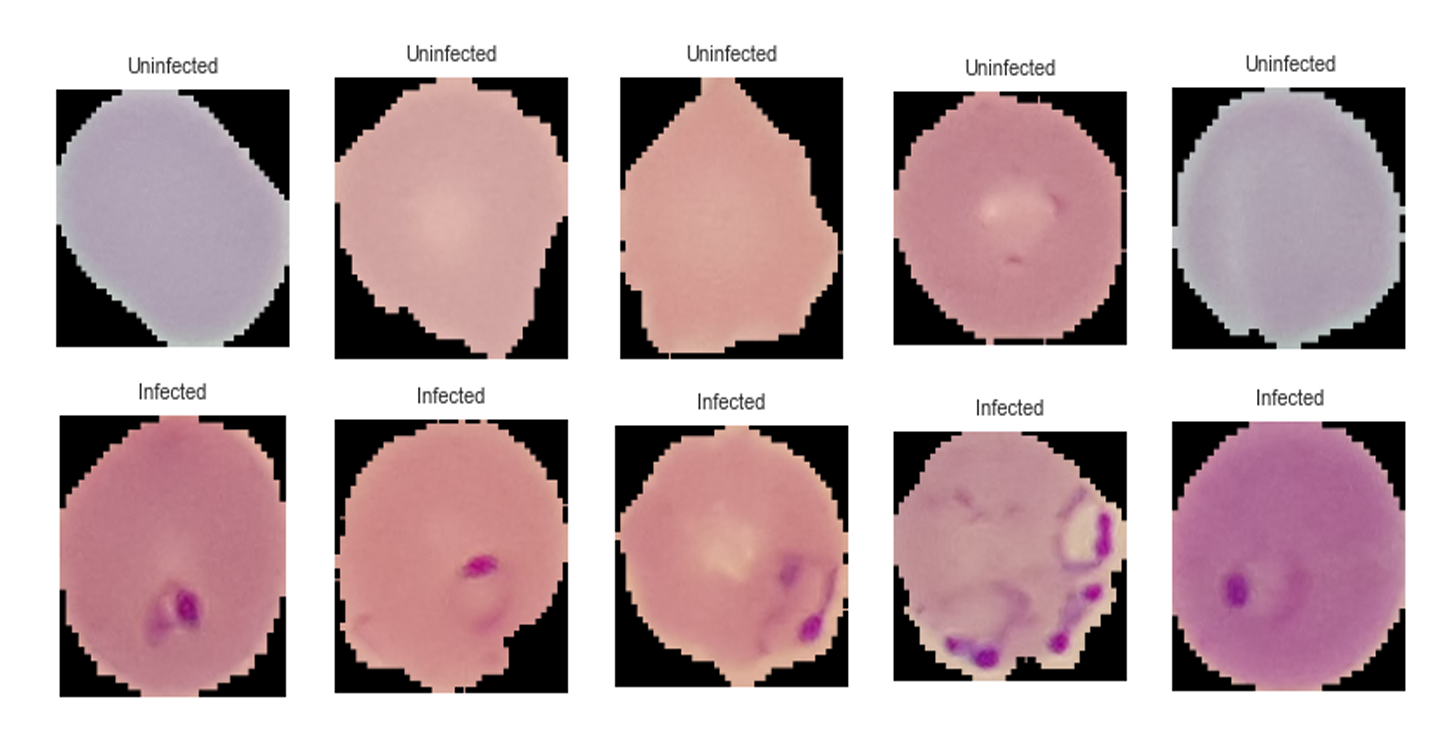
\includegraphics[width=0.8\textwidth]{images/fig1.png}
\caption{Microscopic images from the Dataport dataset showing infected and uninfected cells.}
\label{fig:fig1}
\end{figure}

\begin{figure}[H]
\centering
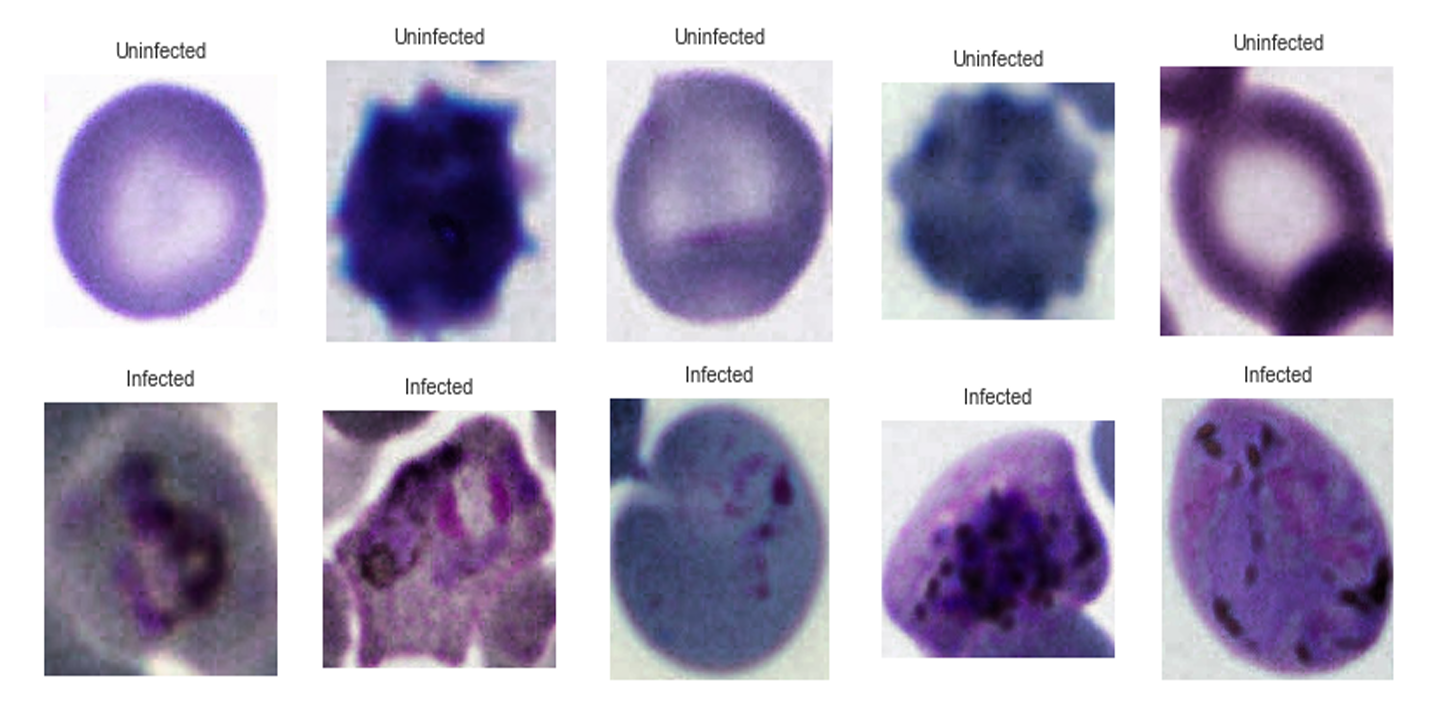
\includegraphics[width=0.8\textwidth]{images/fig2.png}
\caption{Cropped cell images (infected and uninfected) using bounding box annotations from the Kaggle dataset.}
\label{fig:fig2}
\end{figure}

\section{Proposed Method}
In this research, we propose a one-class convolutional autoencoder designed to learn compressed representations of input images belonging to a single class—specifically, microscopic images of malaria cells. This type of autoencoder is trained to reconstruct its input with minimal error, making it particularly effective for anomaly detection by identifying inputs that deviate significantly from the training distribution.

Our proposed autoencoder consists of three main components: an encoder, a latent space, and a decoder. The encoder processes input images—microscopic views of malaria cells—into a lower-dimensional latent representation that captures the most salient features of the data. During training, the autoencoder learns to map normal cell images to a specific region within this latent space, enabling effective differentiation from anomalous inputs.

\begin{figure}[H]
\centering
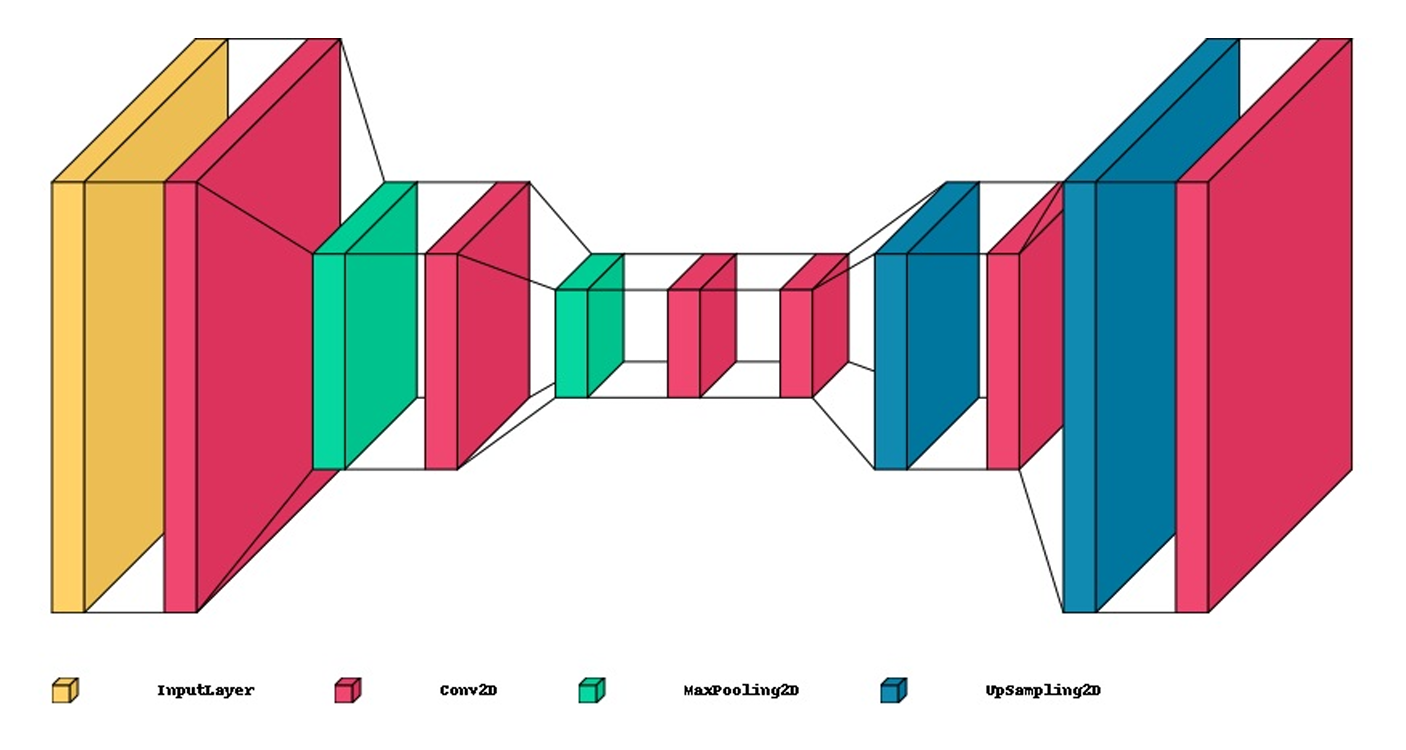
\includegraphics[width=0.8\textwidth]{images/fig3.png}
\caption{Reconstruction of uninfected cell images using an autoencoder.}
\label{fig:fig3}
\end{figure}

Following the encoder, the decoder attempts to reconstruct the original input from the latent representation. The objective is to generate output that closely resembles the input, completing the reconstruction process. To quantify reconstruction accuracy, we use the mean squared error (MSE) as the loss function:

\begin{equation}
MSE = \frac{1}{N}\sum_{i=1}^{N}(x_i - y_i)^2
\end{equation}

where $N$ represents the total number of samples, $x_i$ is the actual value of the $i$-th sample, and $y_i$ is the predicted value of the $i$-th sample \cite{pu2012}.

The model is trained to minimize this loss, encouraging the reconstructed outputs to closely match the original inputs.

During training, the one-class autoencoder is exposed exclusively to normal, non-anomalous data. It learns to accurately reconstruct these inputs, and the latent space is shaped by their distribution. As a result, the model becomes effective at capturing the characteristic patterns of normal cell images.

We use the Structural Similarity Index (SSIM) to evaluate the similarity between original and reconstructed images. During testing, SSIM provides a quantitative measure of how closely reconstructed images of unknown samples match the distribution of known class data. Higher SSIM scores indicate a stronger resemblance, offering insight into the quality of the model’s reconstructions \cite{fu2017}.

According to Wang et al. \cite{wang2009}, the SSIM methodology is based on the principle that the human visual system is especially sensitive to structural information in visual scenes. Preserving this structural detail is therefore essential when assessing image fidelity. SSIM differentiates between two types of distortions: nonstructural and structural. Nonstructural distortions—such as changes in luminance, contrast, gamma, or spatial alignment—typically result from environmental or instrumental factors and do not alter the underlying structure of visual objects. In contrast, structural distortions, including additive noise, blur, and lossy compression, directly degrade the spatial organization of object features within an image.

The SSIM framework is inspired by the human visual system, which is modeled as an ideal information extractor capable of recognizing objects under various types of distortion. Accordingly, SSIM emphasizes sensitivity to structural distortions while compensating for nonstructural ones. The index operates on local image patches (denoted as $x$ and $y$) from two compared images. It evaluates similarity based on three components: luminance $l(x, y)$, contrast $c(x, y)$, and structural correlation $s(x, y)$. These components are computed using simple statistical measures and then combined to produce a local SSIM score, $S(x, y)$.

The SSIM formula is composed of interpretable components that quantify luminance, contrast, and structural similarity between image patches:

\begin{equation}
SSIM(x, y) = \frac{(2\mu_x\mu_y + C_1)(2\sigma_{xy} + C_2)}{(\mu_x^2 + \mu_y^2 + C_1)(\sigma_x^2 + \sigma_y^2 + C_2)}
\end{equation}

Here, $\mu_x$ and $\mu_y$ are the local means of patches $x$ and $y$, $\sigma_x$ and $\sigma_y$ are the corresponding standard deviations, and $\sigma_{xy}$ is the cross-covariance between $x$ and $y$. The constants $C_1$ and $C_2$ are small positive values introduced to stabilize the division when denominators are close to zero.

The SSIM index exhibits symmetry ($S(x, y) = S(y, x)$) and is bounded within the range of -1 to 1. A score of 1 indicates perfect similarity between the compared patches. The index operates within a sliding window, yielding an SSIM map, and the overall image SSIM score is computed—often by averaging SSIM values across the image. Adaptive space-variant weighting and scale-based computations enhance its performance across various spatial scales.

In our approach, classification is based on a predefined SSIM threshold, which is selected according to an acceptable false negative rate (FNR) specified by the practitioner. This threshold is determined using the validation set and the autoencoder’s reconstructed images. A histogram is generated to compare SSIM-based reconstruction errors for normal and anomalous validation samples. We then select a threshold such that most normal images exhibit reconstruction errors above this value, maximizing the model’s ability to distinguish normal from anomalous inputs.

For each test sample, a reconstruction error based on SSIM is computed. If this error exceeds the predefined threshold, the sample is classified as belonging to the normal class. Conversely, samples with errors below the threshold are considered anomalous. This approach provides a principled decision boundary, enhancing the reliability of the classification process.

Accordingly, using a predefined threshold \( \varepsilon \), test samples are classified according to the following decision rule:

\begin{equation}
x_t \in \begin{cases} 
\text{known class,} & \text{if } \varepsilon_t < \varepsilon \\
\text{unknown class,} & \text{otherwise}
\end{cases}
\end{equation}

The threshold \( \varepsilon \) is typically determined by the user based on an acceptable false negative rate (FNR).

In summary, our proposed method employs a one-class autoencoder trained to reconstruct normal microscopic images of malaria cells. This enables the model to identify anomalous or infected instances during testing, demonstrating its potential to improve the accuracy of malaria diagnosis.

\begin{figure}[H]
\centering
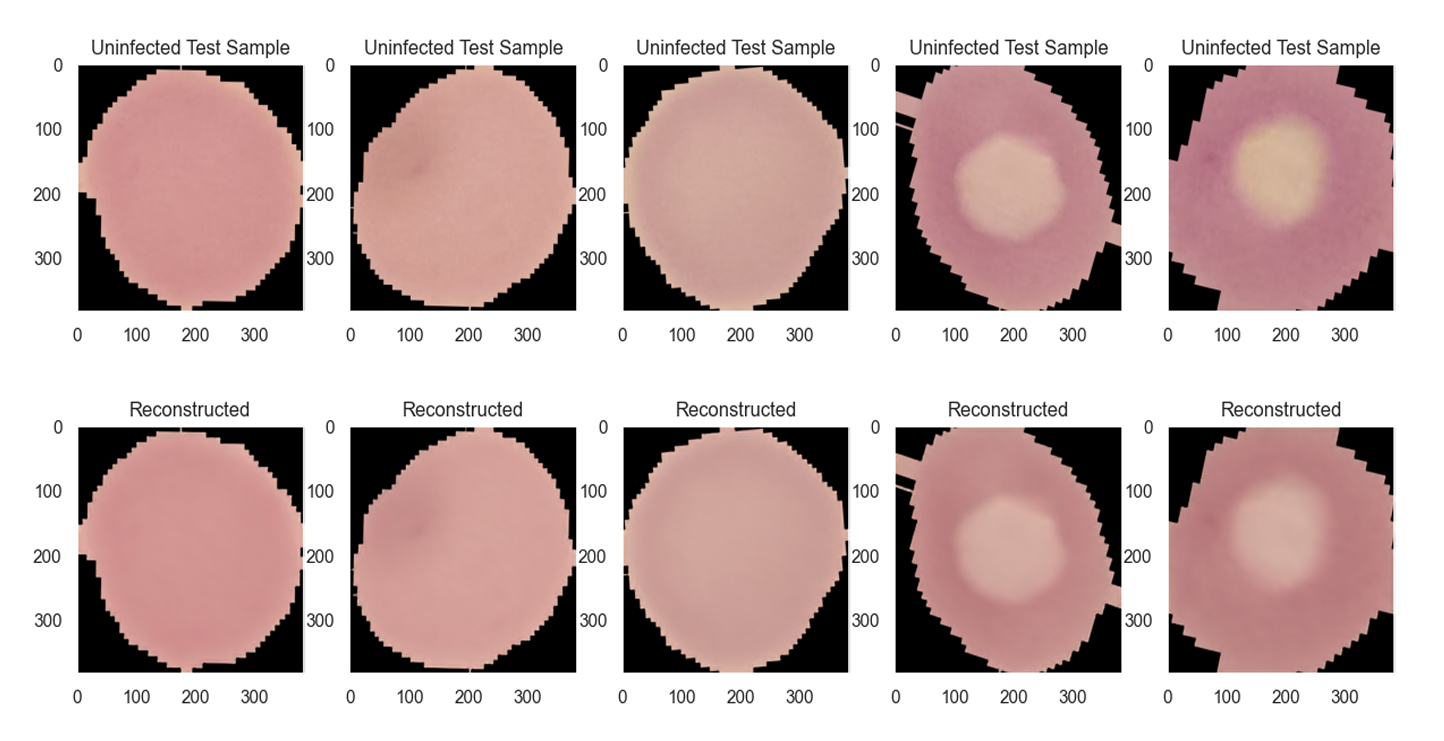
\includegraphics[width=0.8\textwidth]{images/fig4.png}
\caption{Reconstruction of uninfected cell images from the IEEE Dataport dataset using an autoencoder.}
\label{fig:fig4}
\end{figure}

\section{Results}
To assess the effectiveness of our proposed method, we evaluated the model using several performance metrics that quantify accuracy and classification quality:

\begin{figure}[H]
\centering
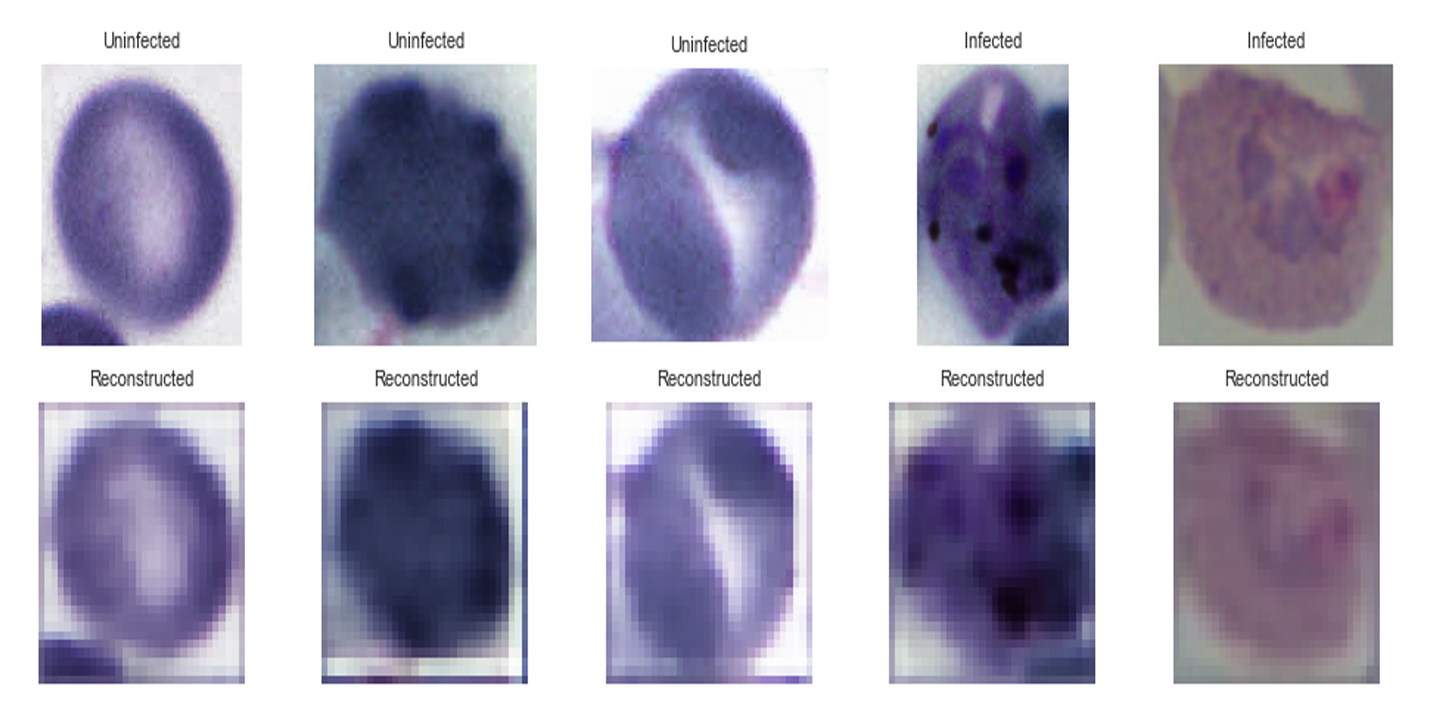
\includegraphics[width=0.8\textwidth]{images/fig5.png}
\caption{Reconstruction of cell images from the Kaggle bounding box dataset using an autoencoder.}
\label{fig:fig5}
\end{figure}

SSIM was selected as an evaluation metric because it captures both global and local features in reconstructed images, emphasizing perceptual similarity. This makes it well-suited for assessing how effectively the model preserves critical visual structure. Integrating SSIM with thresholding improves the method’s precision and robustness when classifying malaria-infected cells in microscopic images, supporting its utility in medical diagnostics.

To determine the most effective evaluation metric for distinguishing normal and abnormal cell images, we compared mean squared error (MSE) and structural similarity index (SSIM). Our goal was to identify a metric that supports high classification accuracy while minimizing false positive rates.

MSE performed poorly in classifying malaria cell images. This limitation is well documented in the work of Wang et al. \cite{wang2009}, who demonstrated the shortcomings of MSE and the advantages of SSIM as an image evaluation metric.

According to Wang et al. \cite{wang2009}, mean squared error (MSE), while effective as a loss function, has several limitations when used as an image evaluation metric.

\textbf{Lack of Sensitivity to Human Perception:} MSE does not reflect how humans perceive visual differences. It treats all pixel errors equally, ignoring that some discrepancies are more perceptually significant than others. For example, small errors in smooth regions may go unnoticed, while similar errors in textured or high-contrast areas are more apparent. This failure to account for perceptual salience leads to inaccurate assessments of image quality.

\textbf{Inability to capture structural information:} Images contain structural elements—such as edges, textures, and spatial patterns—that are crucial for human perception. MSE treats images as collections of independent pixels and fails to account for spatial relationships among features. Even when pixel values remain constant, changes in these relationships can significantly affect perceived image quality.

\textbf{Failure to address image content-dependent variations:} MSE treats all pixels equally, regardless of their perceptual relevance. In many images, certain regions—such as faces in portraits—carry greater visual significance than others. This uniform weighting prevents MSE from accounting for differences in how viewers prioritize visual information.

\textbf{Neglect of error signal characteristics:} MSE does not account for the structure of the error signal, such as its correlation with the original image or the sign (positive or negative) of pixel-wise errors. In real-world scenarios, these errors are often content-dependent, and their directionality can influence visual perception. MSE’s uniform treatment of all deviations overlooks these important perceptual factors.

These limitations of MSE are addressed by SSIM, which evaluates image quality using perceptual principles. Its assessment considers structural and statistical features that align more closely with human visual perception. SSIM evaluates images based on three components:

\textbf{Luminance comparison:} SSIM computes the luminance term by comparing the average pixel intensities of two images. This reflects how the overall brightness of the images corresponds. When the average intensities are similar, it indicates similarity in luminance.

\textbf{Contrast comparison:} The contrast term is calculated by comparing the standard deviations of pixel intensities in each image, which reflects the degree of local variation. Images with similar contrast will exhibit small differences in these standard deviations, indicating a close match in contrast characteristics.

\textbf{Structure comparison:} The structure term measures the correlation between corresponding pixels in the two images, capturing the spatial relationships that define structural similarity. When pixel intensities are strongly correlated in aligned regions, this indicates similar structural organization between the images.

These principles made SSIM the most effective evaluation metric for this task. We evaluated our model using several standard classification metrics:

\textbf{Accuracy:} This metric measures the proportion of correct predictions made by the model. Values closer to 1.0 (or 100\%) indicate stronger overall performance \cite{powers2011}.

\textbf{Recall:} Also known as sensitivity or true positive rate, recall measures a model’s ability to correctly identify all relevant instances—in this case, malaria-infected cells. Missing an infected cell (a false negative) may have serious medical consequences, so maximizing recall for the positive class is critical \cite{powers2011}.

\textbf{Precision:} Precision measures how many of the instances predicted as positive by the model are actually correct. It quantifies the proportion of true positives among all predicted positives \cite{powers2011}.

\textbf{F1 score:} The F1 score is the harmonic mean of precision and recall, providing a single value that balances both metrics. It is especially useful when there is a trade-off between false positives and false negatives, as it captures both the completeness and exactness of the model’s predictions \cite{powers2011}.

\textbf{Specificity:} Specificity measures the proportion of actual negative instances (e.g., non-infected cells) that the model correctly identifies. It reflects the model’s ability to avoid false positives by accurately classifying negative cases \cite{powers2011}.

\subsection{Evaluation Metrics Results}
While the autoencoder did not yield optimal results initially, it effectively minimized loss over the 35 training epochs. The consistent decrease in both training and validation loss indicates successful compression of input data while preserving essential features. Moreover, the absence of divergence between training and validation losses suggests stable learning without signs of overfitting. These outcomes provide a solid foundation for future refinement of the model.

The confusion matrix analysis revealed limitations with the mean squared error (MSE) metric. Specifically, the MSE-based model struggled to distinguish accurately between infected and uninfected cells, exhibiting elevated rates of both false positives and false negatives. As shown in the confusion matrices, this performance reflects MSE’s inability to capture the subtle visual patterns critical for malaria detection. In contrast, the structural similarity index (SSIM)—which incorporates luminance, contrast, and structural features—more effectively captured image-level distinctions. As a result, models evaluated with SSIM demonstrated greater classification accuracy and reliability, making it the more suitable metric for this task.

The model demonstrated strong performance across both the Bounding Boxes Kaggle Malaria dataset and the IEEE Dataport Malaria Dataset. It achieved a recall of 0.97 on the Kaggle dataset and 0.99 on the IEEE dataset, indicating a high true positive rate in identifying malaria-infected cells. These results highlight the model’s effectiveness in detecting abnormal instances and provide a basis for further refinement.

\begin{figure}[H]
  \centering
  \begin{minipage}{0.45\textwidth}
    \centering
    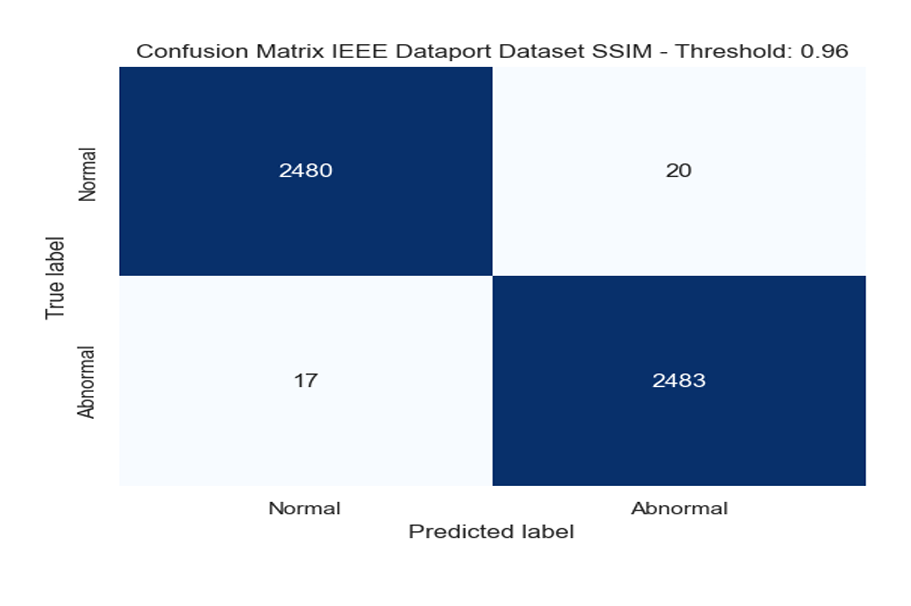
\includegraphics[width=\textwidth]{images/fig6.png}
    \caption{Confusion matrix (SSIM, threshold = 0.96).}
    \label{fig:fig6}
  \end{minipage}\hfill
  \begin{minipage}{0.45\textwidth}
    \centering
    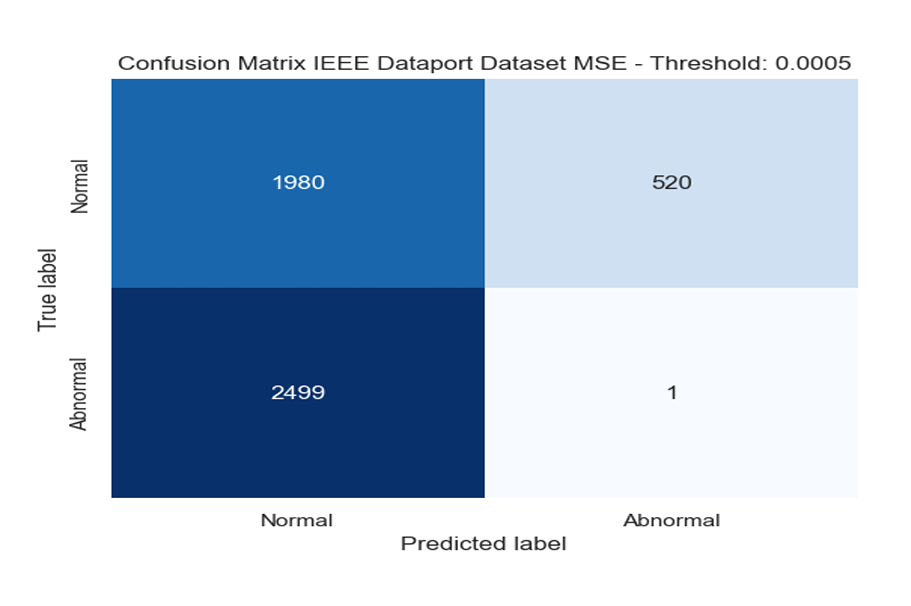
\includegraphics[width=\textwidth]{images/fig7.png}
    \caption{Confusion matrix (MSE, threshold = 0.0015).}
    \label{fig:fig7}
  \end{minipage}
\end{figure}
  
\begin{figure}[H]
  \centering
  \begin{minipage}{0.45\textwidth}
    \centering
    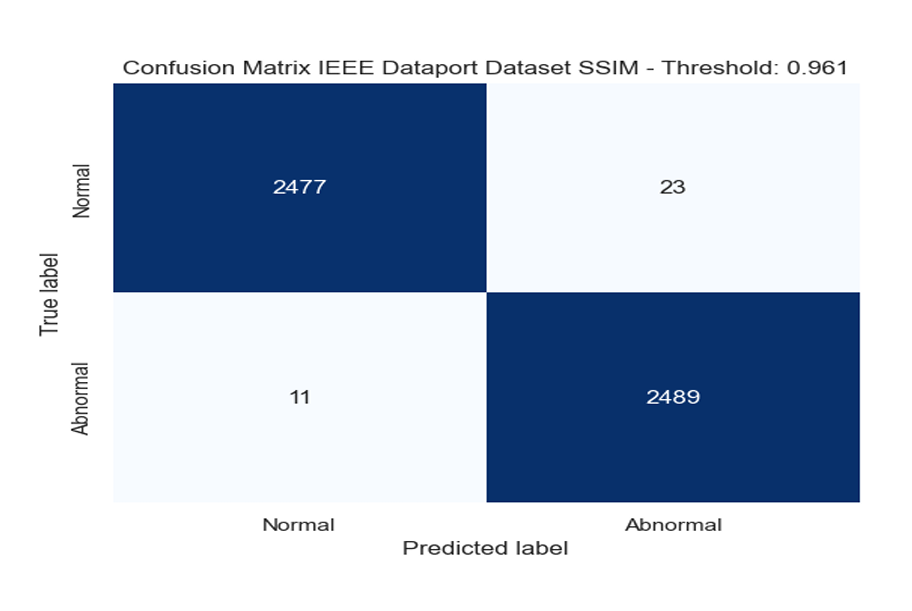
\includegraphics[width=\textwidth]{images/fig8.png}
    \caption{Confusion matrix (SSIM, threshold = 0.961).}
    \label{fig:fig8}
  \end{minipage}\hfill
  \begin{minipage}{0.45\textwidth}
    \centering
    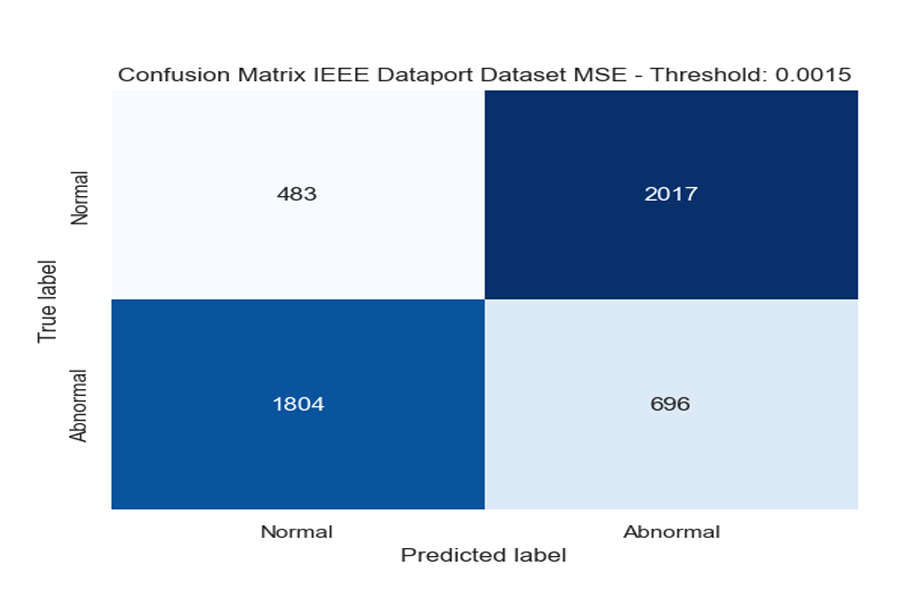
\includegraphics[width=\textwidth]{images/fig9.png}
    \caption{Confusion matrix (MSE, threshold = 0.0025).}
    \label{fig:fig9}
  \end{minipage}
\end{figure}
  
\begin{figure}[H]
  \centering
  \begin{minipage}{0.45\textwidth}
    \centering
    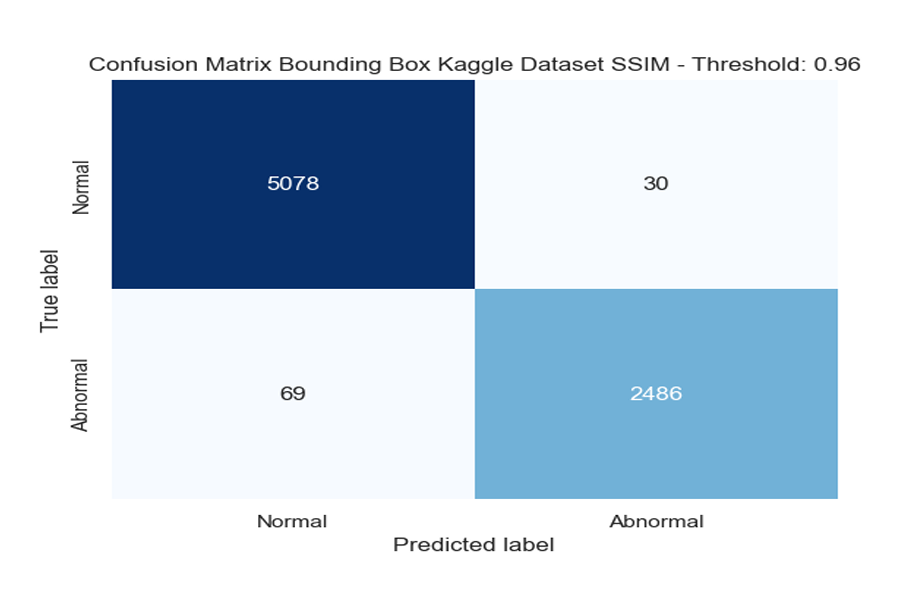
\includegraphics[width=\textwidth]{images/fig10.png}
    \caption{Confusion matrix (SSIM, threshold = 0.96).}
    \label{fig:fig10}
  \end{minipage}\hfill
  \begin{minipage}{0.45\textwidth}
    \centering
    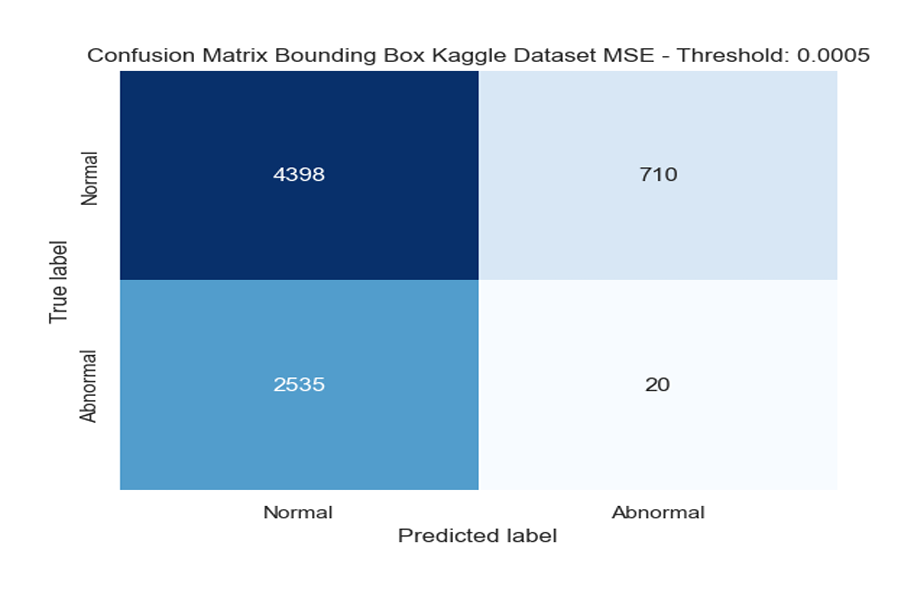
\includegraphics[width=\textwidth]{images/fig11.png}
    \caption{Confusion matrix (MSE, threshold = 0.0035).}
    \label{fig:fig11}
  \end{minipage}
\end{figure}

\begin{figure}[H]
  \centering
  \begin{minipage}{0.45\textwidth}
    \centering
    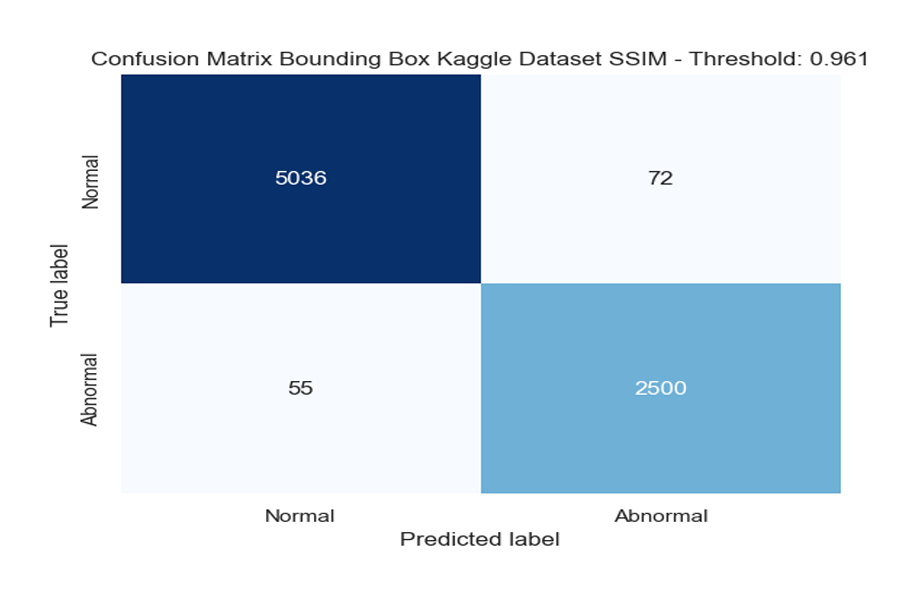
\includegraphics[width=\textwidth]{images/fig12.png}
    \caption{Confusion matrix (SSIM, threshold = 0.961).}
    \label{fig:fig12}
  \end{minipage}\hfill
  \begin{minipage}{0.45\textwidth}
    \centering
    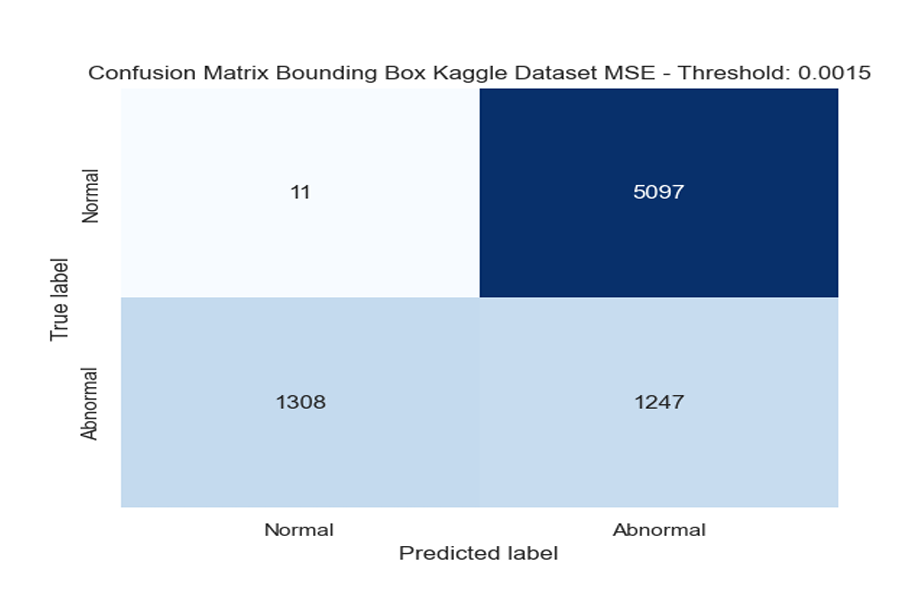
\includegraphics[width=\textwidth]{images/fig13.png}
    \caption{Confusion matrix (MSE, threshold = 0.0045).}
    \label{fig:fig13}
\end{minipage}
\end{figure}
  
\begin{figure}[H]
  \centering
  
\includegraphics[width=\textwidth]{images/fig14.png}
  \caption{Placeholder: Combined SSIM and MSE confusion matrices (figure pending).}
  \label{fig:fig14}
\end{figure}

The precision of 0.99 for both datasets demonstrates the model's strong performance in identifying positive cases. Notably, the recall for abnormal instances is also high—0.97 for the Bounding Boxes Kaggle Malaria dataset and 0.99 for the IEEE Dataport Malaria Dataset. These results indicate that the model correctly identified a large proportion of actual abnormal instances, with 97\% for the former and 99\% for the latter.

The F1-score, which balances both precision and recall, demonstrated strong performance across both datasets—0.98 for the Bounding Boxes Kaggle Malaria dataset and 0.99 for the IEEE Dataport Malaria Dataset. These metrics highlight the model's proficiency in accurately classifying both normal and abnormal instances. Similarly, the overall accuracy of 0.99 underscores consistent performance and further validates the model’s effectiveness in detecting malaria-infected cells.

\subsection{Threshold Identification}
In this research, determining the structural similarity index (SSIM) threshold value was a key step in the evaluation process. This involved analyzing the validation set and plotting the distribution of SSIM scores for normal instances. By selecting a threshold at a point where normal samples were consistently clustered, the model achieved a balance between sensitivity and specificity. This approach enabled the optimization of the true positive rate while reducing false positives.

It is important to emphasize that the performance of any model is closely tied to the dataset and context in which it is applied. The parameters used in this study were selected with consideration for the relatively small sample size. In cases involving larger datasets, alternate parameter settings may be required to maintain optimal performance. The selection of an appropriate SSIM threshold is particularly critical in anomaly detection, as it directly affects the model’s ability to distinguish between normal and abnormal instances. A threshold set too high may result in false negatives—overlooking anomalous cases—while a threshold set too low may increase false positives by misclassifying normal instances. To mitigate these risks, the methodology employed here involved visual analysis of SSIM distributions and careful threshold tuning to balance sensitivity and specificity, ensuring the model’s reliability in practical applications.

\begin{figure}[H]
\centering
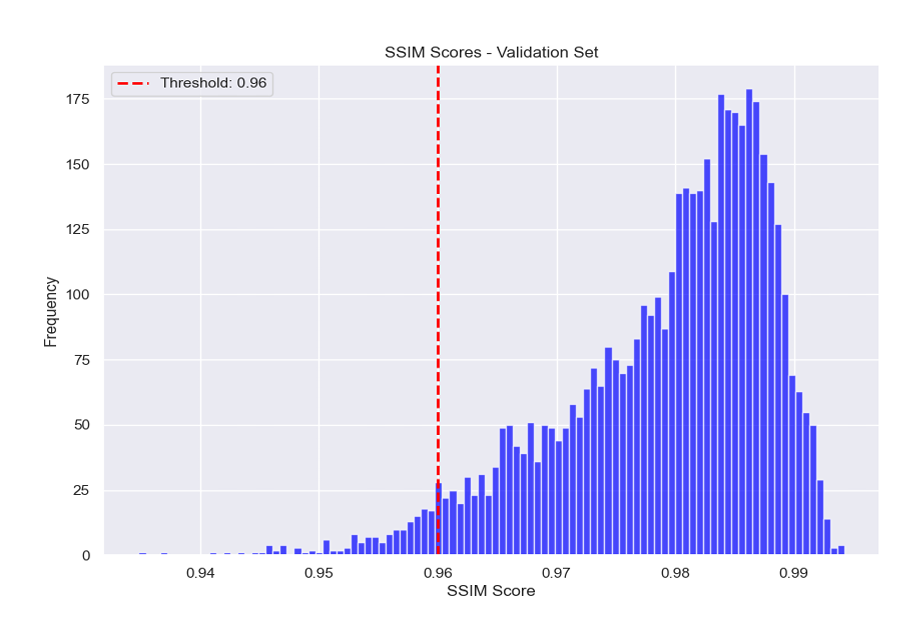
\includegraphics[width=\textwidth]{images/fig15.png}
\caption{SSIM threshold selection for IEEE Dataport dataset (threshold chosen above 0.96).}
\label{fig:fig15}
\end{figure}

\begin{figure}[H]
\centering
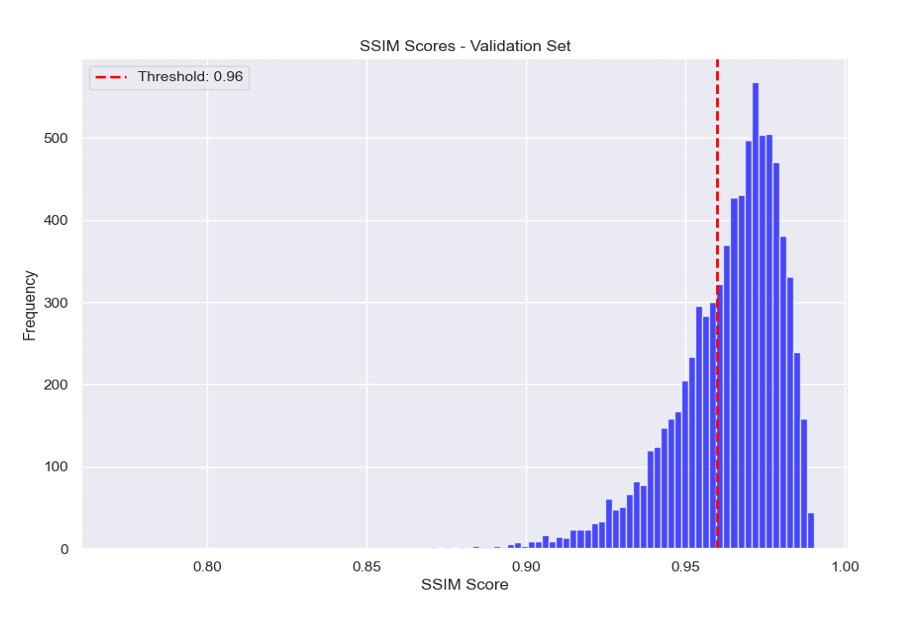
\includegraphics[width=\textwidth]{images/fig16.png}
\caption{SSIM threshold selection for Bounding Box Kaggle dataset, with threshold chosen above 0.96.}
\label{fig:fig16}
\end{figure}

\begin{table}[H]
  \caption{Evaluation metrics across various models and datasets.}
  \label{table:eval_metrics}
  \centering
  \begin{tabular}{l|c|c|c|c|c}
    \hline
    \textbf{Metric} &
    \makecell[c]{OC Autoencoder\\(IEEE Dataport)} &
    \textbf{Autoencoder} &
    \textbf{CNN} &
    \makecell[c]{Transfer\\Learning} &
    \makecell[c]{OC Autoencoder\\(Bounding Boxes)} \\
    \hline
    Accuracy & 0.99 & 0.9531 & 0.9728 & 0.948 & 0.99 \\
    Recall (Sensitivity) & 0.99 & 0.9528 & 0.9515 & -- & 0.97 \\
    Specificity & 0.99 & -- & 0.9962 & -- & 0.99 \\
    Precision & 0.99 & 0.9626 & 0.9960 & -- & 0.99 \\
    F1-score & 0.99 & 0.9577 & 0.9732 & -- & 0.98 \\
    \hline
  \end{tabular}
\end{table}

\section{Conclusion}
Malaria is a life-threatening disease, and early diagnosis is critical for saving lives. The accuracy of malaria detection from blood smear images often depends on the skill of medical professionals and the quality of available diagnostic tools. This dependency can place a significant burden on healthcare providers in rural areas with limited medical infrastructure. Deep learning methods that offer high diagnostic accuracy can help alleviate this strain by improving the speed and reliability of the diagnostic process. The proposed one-class autoencoder method shows promise as an effective decision-support tool for medical practitioners, particularly in resource-limited settings.

In addition, the proposed method—a one-class autoencoder—addresses a common limitation in many classification models: the scarcity of abnormal instances. Because the autoencoder is trained exclusively on normal images, it learns to identify abnormalities by detecting deviations from the learned distribution. This approach enables the model to achieve high accuracy even when trained on a relatively small dataset of normal instances.

\newpage
\bibliographystyle{IEEEtran}
\bibliography{references}
\end{document}